VeriPlace had already profiled and templated an inherently distributed architecture with built-in privacy awareness, taking a first infrastructural step towards defending against proxy attacks, without the need for trusted hardware \cite{luo2010veriplace}. The whole setup is especially tangled and consequently resourceful for the levels of trust it assumes, but it definitely settled the ground for the next generation of \pol{} schemes. 

\begin{figure}[ht]
    \begin{center}
    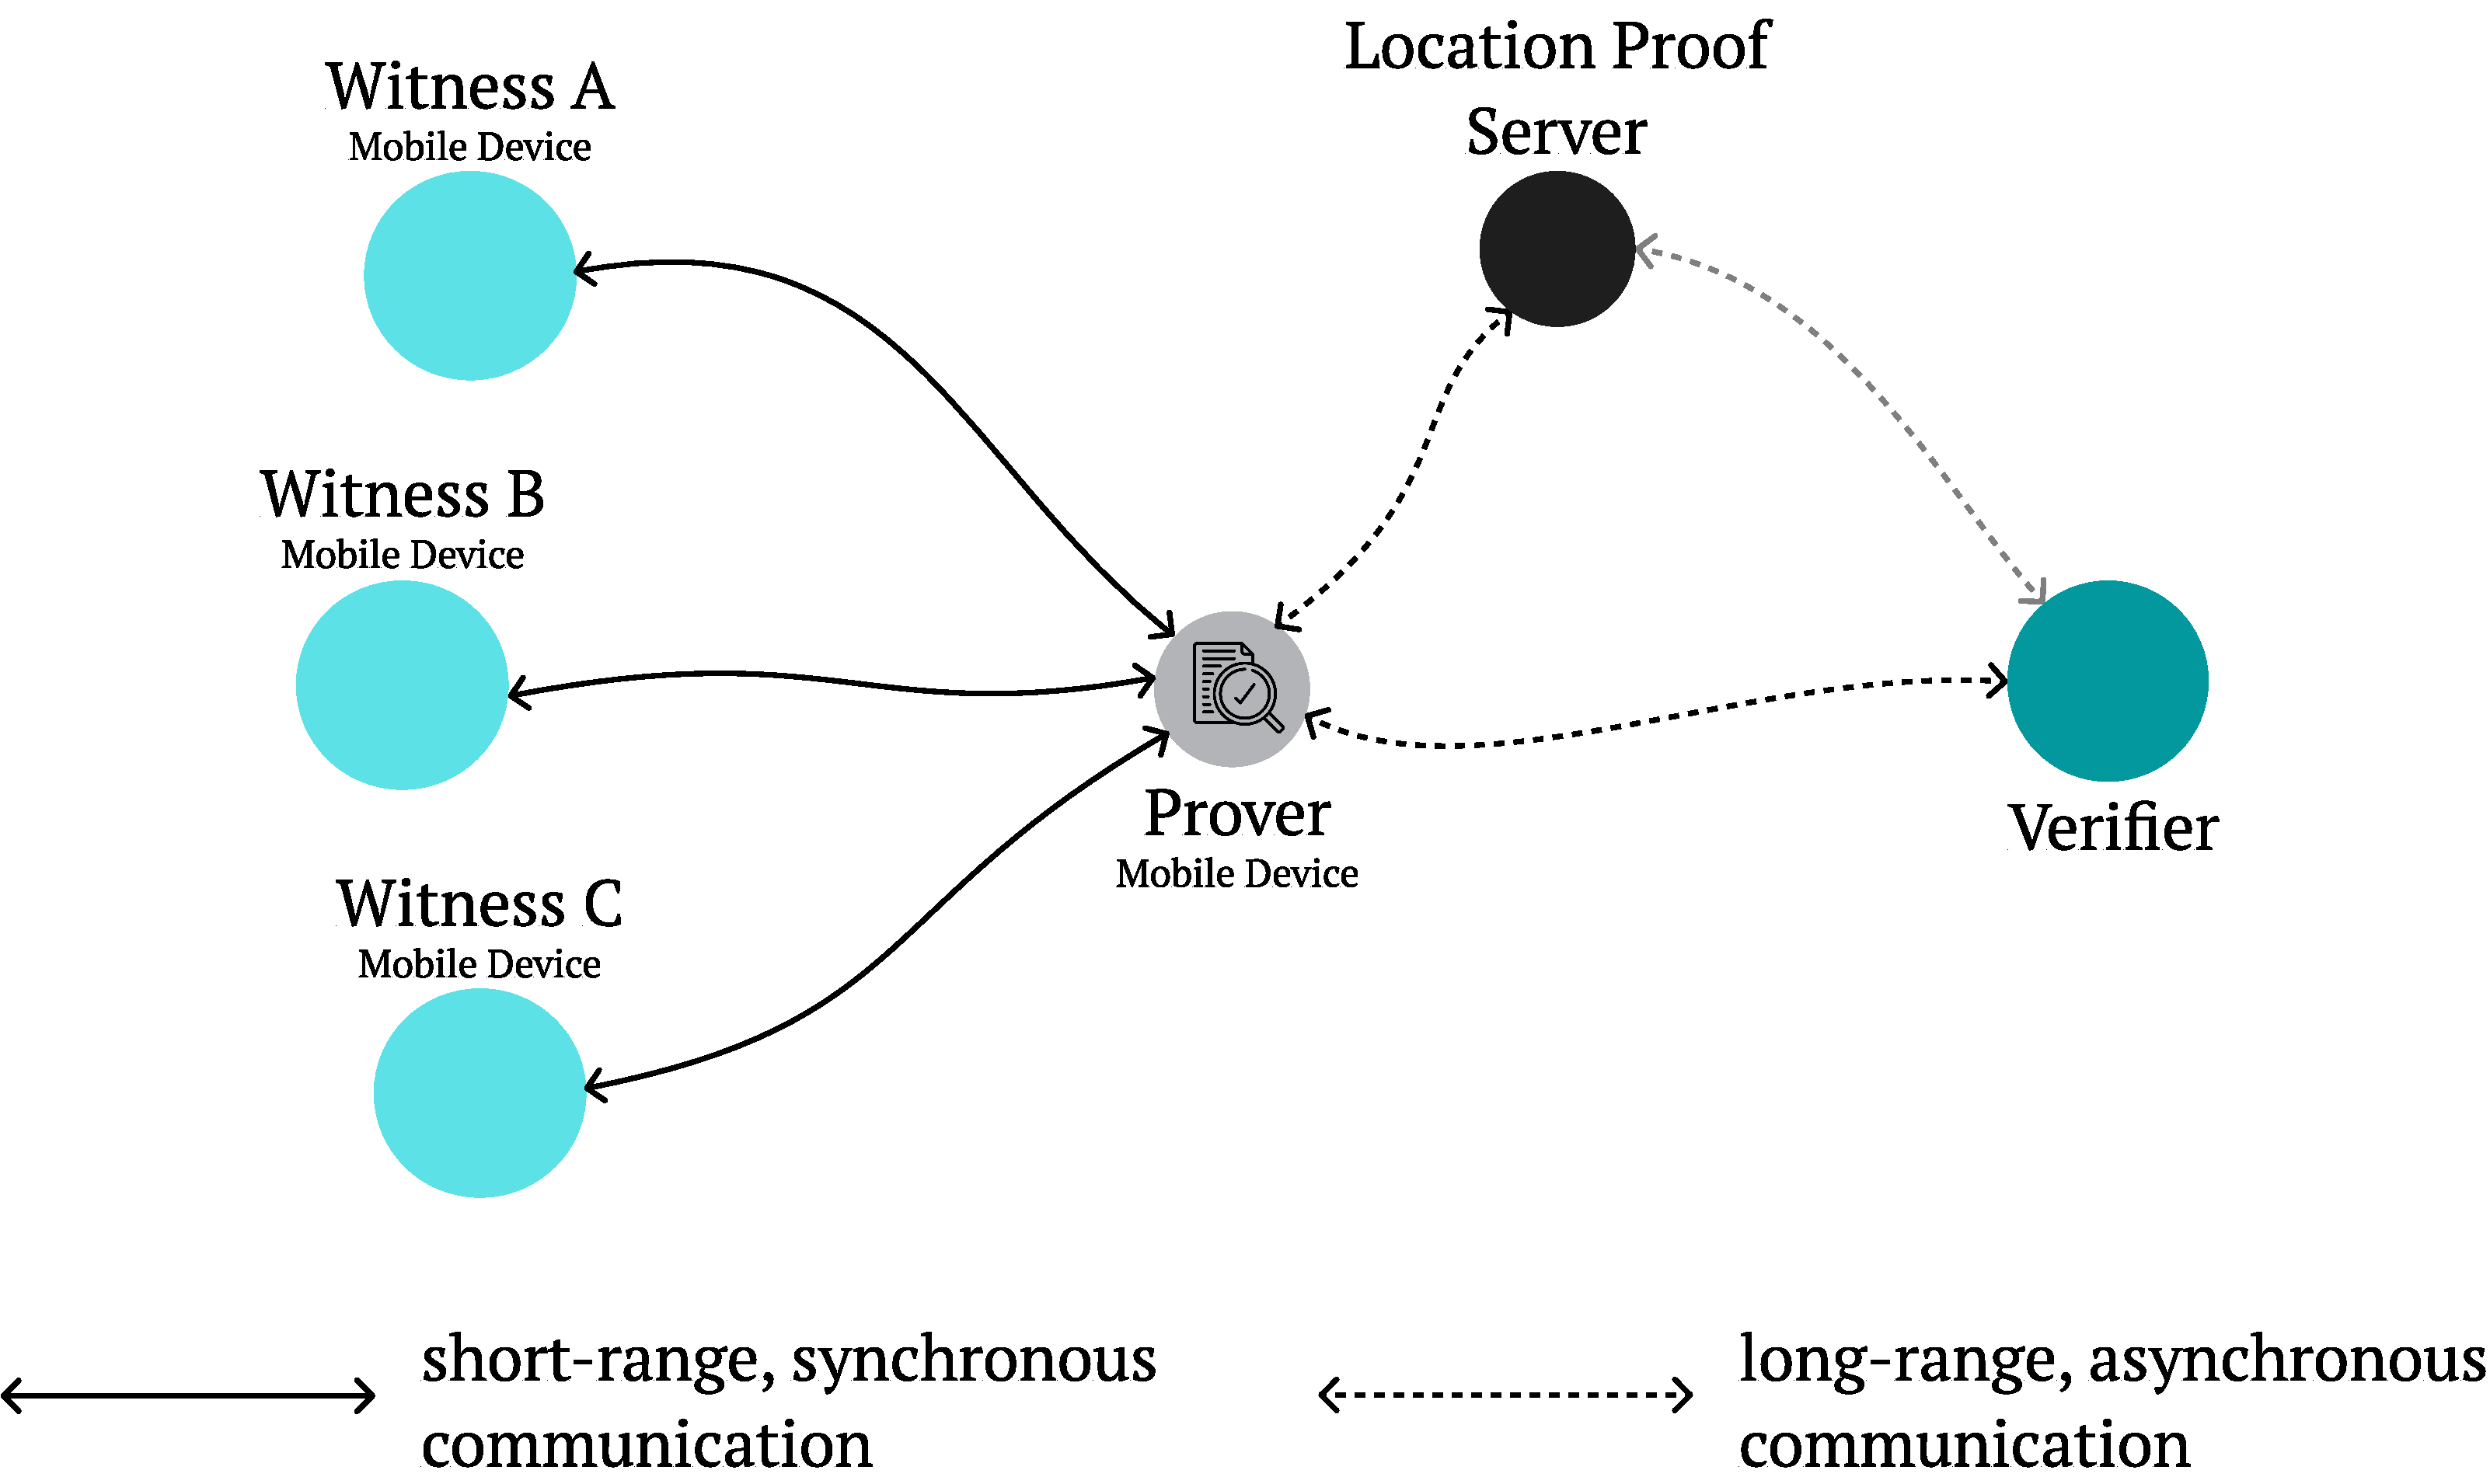
\includegraphics[width=0.9\textwidth]{decentralized-pol.pdf}
    \caption{APPLAUS, by Zhu and Cao \cite{zhu2011applaus}, envisions the prover to communicate individually, via Bluetooth, with nearby witnesses. Each witness should agree on providing a location proof, upon the prover's request, to be submitted later to an untrusted location proof server. This server will store the location proof historic records, to be queried by the verifier, in order to assert a prover's location within a specific time period. The prover, witnesses, and verifier are all assumed to be trusted by each other, leaving out the location proof server.}
    \label{fig:decentralized-pol}
    \end{center}
\end{figure}

The following evolutionary stage of these protocols aims at flexing and distributing trust, resources, power, and responsibility, with the hope of achieving more resilient, fault-tolerant, and scalable systems. APPLAUS, by Zhu and Cao \cite{zhu2011applaus}, delivers one of the first distributed protocols that combines the location proof and location privacy problems. It uses Bluetooth enabled mobile devices that communicate with nearby participants, during the proof generation process. The protocol asserts certain bond levels between the \emph{prover}, \emph{verifier}, and \emph{witnesses}, all of them known to a trusted Certificate Authority (CA), disregarding, on the other hand, the need for a fully trusted location proof server to store the historic location records (see Figure~\ref{fig:decentralized-pol}). The claim is that, by statistically changing the pseudonyms for each device and by following a user-centric privacy model, the protocol can effectively generate privacy preserving location proofs and store them in a trustless manner. STAMP \cite{wang2016stamp} and PROPS \cite{gambs2014props} are two contemporaneous works that take the same witnessing approach as APPLAUS, but follow the path of convincing the verifier by presenting several shares of a composite location proof, based on group signatures. Both of them try to more profoundly tackle the prover's and witnesses' privacy concerns, but may admittedly fail at preventing collusion scenarios between them. Gambs et al. argue that the reliance on a trusted third party may be an unavoidable requirement, even if against the authors' principles of location sovereignty, especially when one wants to entirely prevent unbounded collusion attacks \cite{gambs2014props}. SPARSE, by Nosouhi et al. \cite{nosouhi2018sparse}, avoids the typical distance-bounding mechanism and the witness picking process by the prover, as done in the previous works, with the goal of protecting against those collusion attempts, at best, in relatively crowded and decentralized witnessing situations. 

At this point, all these schemes have assumed the common goal of protecting the identity of the parties involved in the proof generation process, but they have not yet tackled the additional problem of keeping the location information proportionally private from whoever needs to verify it. Dupin et al. \cite{dupin2018location} theoretically propose a Secure Multi-Party Computation (SMPC) based protocol that is provably resilient against any semi-honest participant. Their solution could still benefit from the classical distance-bounding mechanisms \cite{dupin2018location}, but it is highly resourceful and practically infeasible, as it relies on expensive and complex cryptographic primitives and assumes directional antennas \cite{yang2021group}.

On the horizon of these solutions was still the high level need for detaching \pol{} protocols from any kind of trusted central authority, for both identity and information management. This goal has naturally met, along the way, Blockchain technology. The next section will finally present the most recent developments in achieving decentralized, trustless, and infrastructure-independent \pol{} schemes.
